\chapter*{\FontH{\Huge Die Maus mit den drei Federn}}
\addcontentsline{toc}{chapter}{Die Maus mit den drei Federn}
\lettrine[lines=3]{\color{DeepPink}E}{ine} Mause lebte viele Jahre sehr bequem in einer Mühle, die einem alten Müller gehörte. Der konnte nicht mehr sehr gut sehen, was das Leben der Maus sehr einfach machte. Das beste war, dass immer genügend Weizenkörner herumlagen, die der Alte verschüttet hatte, so dass die Maus nie Hunger leiden musste. Ausserdem konnte der Müller die Maus nie fangen, mit seinen trüben Augen. Eigentlich wusste die Maus aber, dass er das auch gar nicht wollte, denn so war er nicht so alleine in seiner Mühle. So lebten sie lange nebeneinander her und waren zum Schluss beinahe Freunde. 

Die Maus genoss ihr fürstliches Leben. Egal ob sommers oder winters, ob kalt, ob warm, hier fand sie immer alles, was das Leben schön machte. Und da sie ohne Futtersuche viel freie Zeit hatte, nagte sie an Holzstücken herum, bis diese die lustigsten Formen hatten. Einmal benagte sie sogar ein Stück Kaminholz so, dass es ein exaktes Abbild des Müllers ergab. Aber dieser warf das Holz in seiner Blindheit ins Feuer wie jedes andere Stück Holz auch. Am liebsten aber machte sie Mäusepüppchen, die sie dann an Mäusekinder verschenkte, die nicht so viel hatten wie sie. Die Püppchen gelangen der Maus jedes Mal so gut, dass unfehlbar jede Mutter eines beschenkten Kindes laut seufzte und die Väter ihr Taschentuch zückten und laut schneuzten. 

Eines Tages starb der Müller. Der neue Müller, ein Neffe des Verstorbenen, war leider nicht von schlechtem Auge, wie die Maus schnell feststellen musste. Schon am ersten Tag warf er ihr einen Schuh hinterher. Und noch einen Tag später hatte er zwei widerliche Katzen angeschafft, die nur dafür da waren, sie durch die Mühle zu jagen. Sobald die beiden sich hier besser auskennen würden, überlegte die Maus, würde sie schnell ein schönes Frühstück abgeben.

Der Maus blieb nichts weiter übrig, als die traute Mühle zu verlassen und ihr Glück woanders zu probieren. So wanderte sie durch die Welt. Erst hatte sie Angst, in den fetten Jahren das Mausen verlernt zu haben, aber ein paar Körner fanden sich irgendwo dann doch jeden Tag. So ging es bis der Herbst die Blätter färbte und dem unvermeidlichen Winter die Türen öffnete. Und mit dem Winter kamen die Kälte und der Hunger. Nur noch selten fand sich irgendetwas zum Essen und als der erste Schnee fiel, wurde der Hunger wirklich schlimm. 

Die Maus hatte keinen Vorrat angelegt, daran hatte sie nicht gedacht. Beim Müller in der Mühle war das ja auch nie wichtig gewesen. Da sass sie nun, ohne zu wissen, ob sie schlotterte, weil der Wind ihr den Schnee immer tiefer ins Fell blies, oder weil ihr Bauch so laut brummte, dass man dachte, sie sei ein Bär. Und als sie glaubte, jetzt sei alles vorbei, kam ein kleines Mäusekind mit einem ihrer genagten Mäusepüppchen und sah die Maus in ihrem ganzen Elend.
\afterpage{
    \begin{figure}
        \thispagestyle{empty}
        \centering
        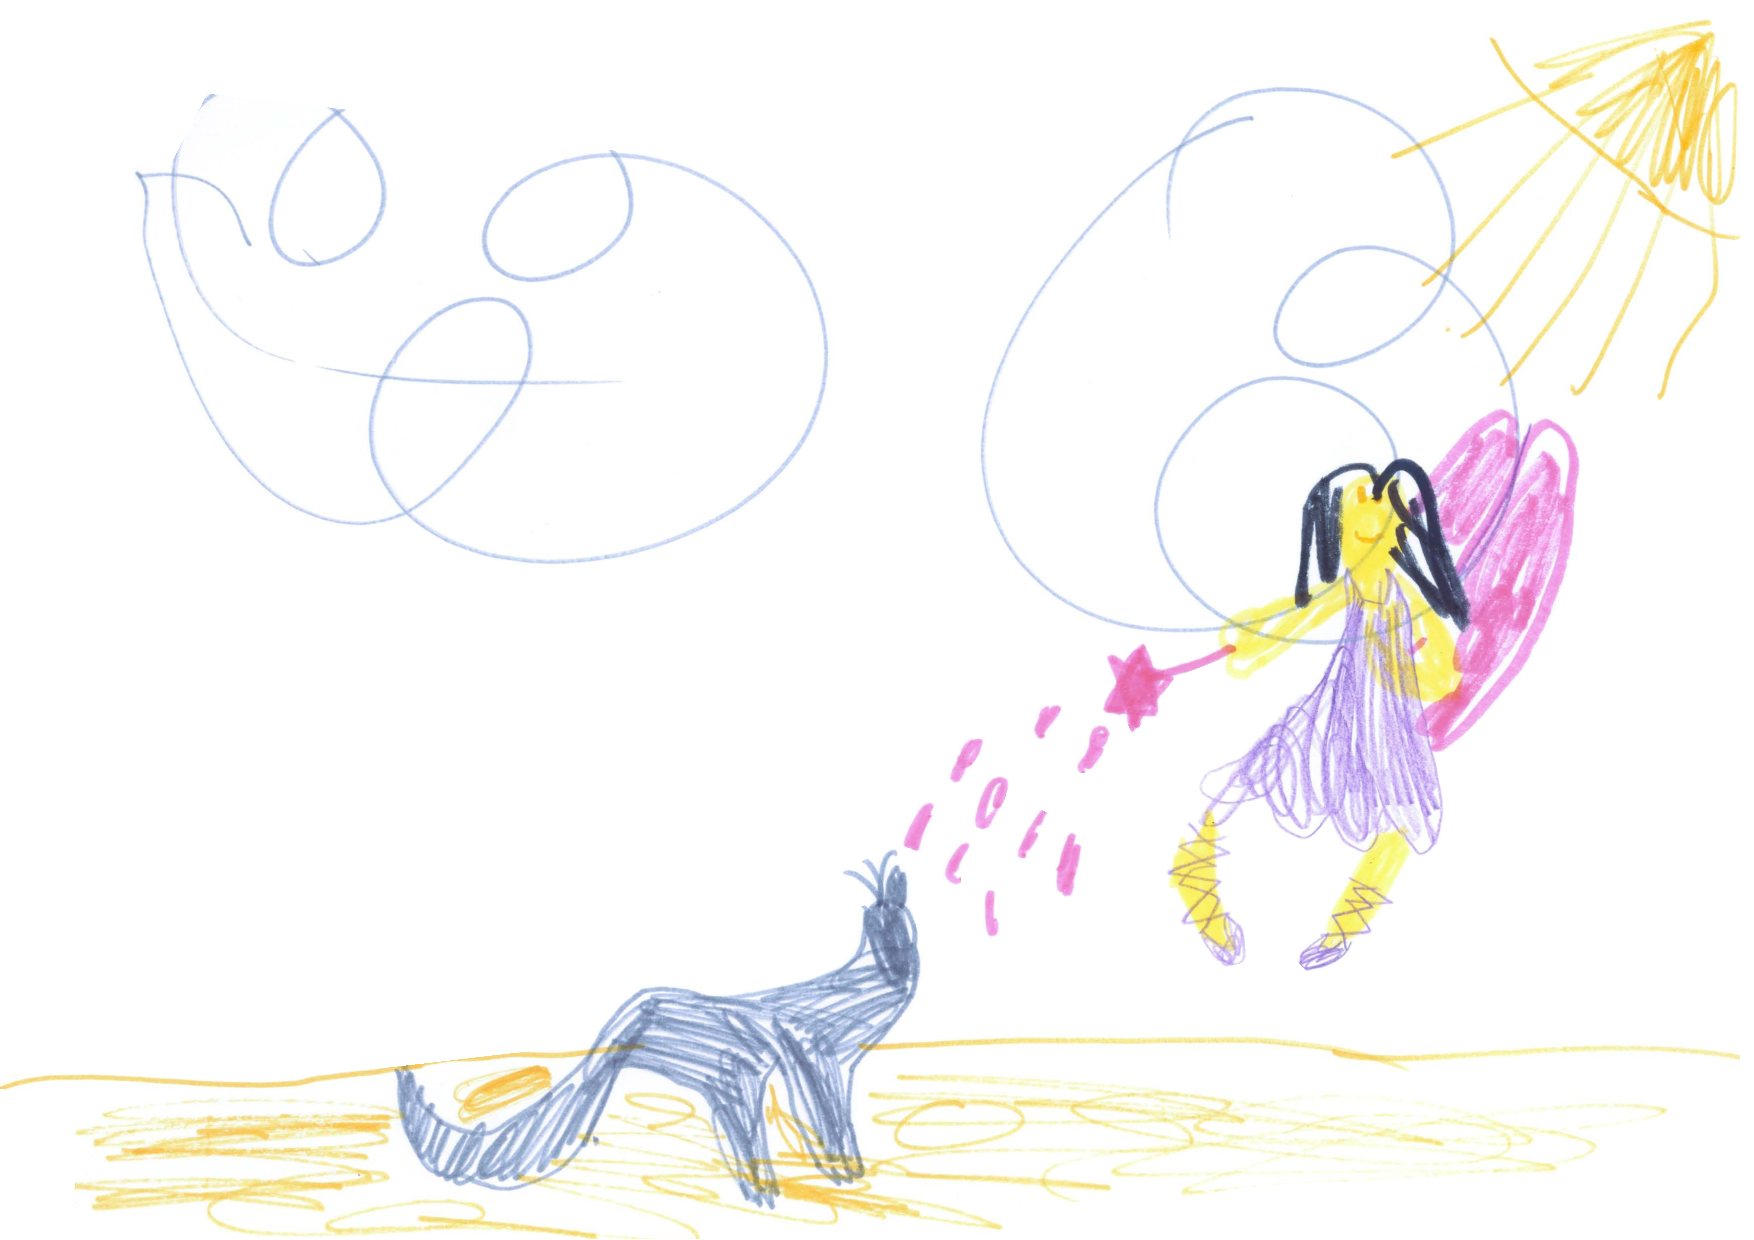
\includegraphics[width=\textwidth]{bilder/1mausFee.pdf}
    \end{figure}
    \clearpage
}

Das Kind war aber gar kein richtiges Mäusekind, sondern eine gute Fee. Und weil sie Mitleid mit der Maus hatte, sagte sie zu ihr: 

\enquote{Du bist eine gute Maus, dass weiss ich. Du hast mir einmal dieses Holzpüppchen geschenkt obwohl du mich gar nicht gekannt hast, und deswegen will ich dir helfen. Leider bin ich keine der mächtigen Feen, die alle Wünsche erfüllen können, aber ich kann dir drei Mal einen guten Rat geben. Nimm dazu diese drei Federn. Wenn du eine auf die Hand legst, und in die Luft bläst, stelle deine Frage und ein Geist wird erscheinen und dir die Antwort geben.}

Die Maus wusste zuerst gar nicht, was für ein grosses Geschenk das war. Was nützen mir Ratschläge, dachte sie zunächst, wenn ich vor Hunger fast nicht denken kann? Aber dann kam der Maus ihre erste Idee. Warum nicht fragen, wo es heute feines Futter zu finden gibt? Und schon hatte sie eine Feder in der Hand. Aber halt, warum nicht gleich fragen, wo es heute und morgen etwas Leckeres gibt, dachte sie richtig. Die Maus wurde immer aufgeregter, als sie langsam verstand, was sie da von der Fee bekommen hatte. Denn noch besser konnte sie fragen, wo es eine Mühle so wie ihre gäbe, wieder mit einem Müller der sie in Ruhe liesse? Oder einen Ort, der war wie ihre Mühle, nur dass es noch feine Kleider umsonst gäbe?

So steigerte die Maus ihren Wunsch immer mehr, bis sie irgendwann zu dem Ergebnis kam, dass nur eine Frage geschickt sein könne. Sie nahm eine der Federn, legte sie auf ihre Hand, so wie es die Fee gesagt hatte und blies sie in den Himmel. Ein sanfter Windhauch nahm die Feder und liess sie steigen und steigen. Die Maus blinzelte ihr hinterher und fragte mit lauter Stimme: 

\enquote{Wie schaffe ich es, eine sehr reiche Maus zu werden?} Als die Feder gerade die Sonne zu berühren schien, antwortete eine ferne Stimme:

\enquote{Du kannst keine Körner sammeln, Du kannst keine Höhle bauen. Und doch bist Du geschickt in manchen Dingen. Erkenne was Du kannst! Aber bedenke: Nur wer bescheiden ist und im Sommer die kleinen Äpfel verschont, wird im Herbst grosse süsse Äpfel ernten können.} 

Die Maus hatte vor Aufregung ihre Barthaare gekräuselt. Enttäuscht von der Antwort, rollte sie die wieder auf, nur um sie gleich hängen zu lassen. Was sollte denn das bitte bedeuten? Sie hatte schon gehofft, einen Ratschlag zu erhalten, der besser verständlich wäre. Traurig senkte sie den Kopf. Ihr Blick viel auf einen dicken Ast und so begann sie zu nagen, nur um nicht so frieren. 

Da kam ein Mäusevater des Weges gelaufen und sah die kleine frisch genagte Babypuppe. 

\enquote{Die ist ja herrlich!}, rief dieser, \enquote{Guter Freund, seit Tagesanbruch bin ich auf der Suche nach einem Weihnachtsgeschenk für meine Kinder, sei so gut, und verkaufe mir deine Arbeit, ich möchte dir auch einen Gulden zahlen.}

Die Maus willigte natürlich sofort ein. Ein ganzer Gulden! Was man dafür alles für leckere Dinge kaufen konnte. Danke, liebe Fee, dachte sie, denn jetzt verstand die Maus den Ratschlag der Fee und wurde Puppenmacher. 

Mit dem ersten verdienten Gulden ging die Maus zum Krämer und bestellte sich den ersten Schweizer Käse in ihrem Leben. Gierig atmete sie den Geruch des alten Hobelkäses ein, als ihr gerade noch der zweite Teil des Rates der Fee einfiel. Bescheiden zu sein und sparen, hiess das wohl. Die Maus gab den teuren Schweizer Käse zurück, nicht ohne nochmals einen tiefen Zug des herrlichen Duftes inhaliert zu haben, und liess sich stattdessen vom Krämer ein trockenes Stück Brot geben. 

Mit dem gesparten Geld ging die Maus zum Holzhändler und kaufte sie ein schönes Stück edlen afrikanischen Holzes, ganz in schwarz. Der Holzhändler lachte zunächst, als er die verlumpte Maus sah, die auch noch vom teuersten Holz kaufen wollte. Als diese ihm aber fast einen ganzen Gulden auf den Tisch zählte, schüttelte er nur den Kopf und holte ein Stück Ebenholz. Die Maus begann zu nagen und nagte eine herrliche Büste einer schönen Mäusin. Sie klopfte an alle Türen des Dorfes und konnte die schwarze Schönheit endlich für acht Gulden an einen Kutschenbauer verkaufen.

Wieder sparte sie und kaufte Holz. Daraus nagte sie die schönsten Dinge. Spielzeug und Möbel, Statuen berühmter Mäuse und sonst noch allerlei. Damit zog sie von Haustür zu Haustür und erzielte immer viel mehr Geld, als das Holz gekostet hatte. Nach einem halben Jahr war sie es Leid die Leute zu besuchen und mietete sich ein eigenes Geschäft. Dort konnte sie einen grossen Vorrat an Nagwerk vorrätig halten, da konnte fast jeder etwas passendes finden.

So verging die Zeit und Maus wurde immer reicher. Die edelsten Käse waren eine Selbstverständlichkeit geworden und zwar reichlich. Sie hatte jetzt auch Gehilfen, denen sie gezeigt hatte, wie man nagen muss, das machten die jetzt für sie. Die Maus wurde immer fetter und fetter und fetter, bis sie fast keine Luft mehr bekam. Der herbeigerufene Arzt beschnüffelte die Maus von allen Seiten und prophezeite ein baldiges Herzversagen, wenn das mit der Bauchwachstum nicht schleunigst umgekehrt werden würde, die Maus also abnehmen solle. Aber viel Hoffnung habe er nicht, musste er einräumen.

Die Maus fühlte, dass es Zeit für die zweite Frage sei. Aber was genau sollte sie diesmal fragen? Wie sie ihre Gesundheit retten könne, war sicher eine gute Frage. Aber dann hatte sie nur noch eine Frage übrig und war es nicht sehr gefährlich, diese letzte Frage nicht optimal zu nutzen? Sollte sie nicht vielleicht besser fragen, was die beste letzte Frage sein könne? Möglicherweise war ja aber gerade die Frage nach der Gesundheit die beste Frage. Und dann hätte sie die letzte Frage verschenkt.

Die Maus dachte lange nach, doch konnte sie sich nicht entscheiden. Aber eine Entscheidung musste getroffen werden.  So nahm sie die zweite Feder und blies sie in die Luft. Die zweite Feder erreichte den Mond und gerade als sie diesen berührte, donnerte auch wieder die selbe Stimme wie beim ersten Mal.

\enquote{Also Maus, stelle deine Frage!} Die Maus erklärte ihr Problem, dass sie sich nämlich nicht entscheiden können.

Die Stimme seufzte, murmelte etwas davon, dass es so ja wohl nicht ginge, dass die Maus schon eine klare Frage formulieren müsse, dann aber sprach sie: \enquote{Die Lösung auf beide Fragen sind ein paar gute Schuhe.}

Wie das erste Mal auch, wurde die Maus nicht recht schlau aus diesem Rat. Schuhe? Was konnte das bedeuten? Schuhe hatte sie keine mehr, seitdem sie den eigenen Laden aufgemacht hatte. Wozu auch? Die Mäuse kamen zu ihr, auch der Holz- und der Käselieferant. Es hatte einfach keinen Grund mehr gegeben, das Haus zu verlassen. Dann verstand sie. Na klar, es war gemeint, dass sie laufen solle. Mit einem kleinen Spaziergang war es wohl nicht getan. Also schloss die Maus ihren Laden ab und hängte ein Schild ins Schaufenster, auf dem zu lesen war, dass die Maus jetzt einmal Ferien hat und auf Wanderschaft geht.

Wohin ist egal, dachte sie ganz richtig, Hauptsache laufen. Die Wege führten sie weit weg von zu Hause. Die ersten Tage kam sie dick und ungeübt wie sie war, kaum voran. Aber schon bald war sie wieder bei Kräften und lief eifrig nicht nur die Berge runter, sondern auch wieder hoch.

Die Maus wanderte viele Wochen. Abends klopfte sie an fremde Türen und bat um Unterkunft für eine Nacht. Als Gegenleistung nagte sie ihre berühmten Püppchen oder andere Dinge. So lernte sie die unterschiedlichsten Mäuse kennen. Mal schlief sie bei einer Familie, mal bei einer alten Witwe. Mal waren es wohlhabende Mäuse, mal arme. Eine Maus war sehr schlau und las viel, eine andere kaute den ganzen Tag auf einem Grashalm und machte nur das mindeste.

Alle, die die Maus traf, erzählte sie ihre Geschichte und wollte wissen, welche Frage sie wohl stellen würden. Vielleicht hatten die anderen Mäuse ja eine Idee.

\enquote{Ich würde gerne wissen, welches Mittel es gibt, dass meine Kinder mich einmal eine Nacht schlafen lassen.} wollte eine Mutter wissen. \enquote{Woher weiss ich, ob meine Freundin mich liebt?} war ein jugendliche Maus besorgt. \enquote{Wo bekomme ich den besten Preis für meine Ware?} gab sich ein Händler sachlich. Sehr weit kam die Maus und lernte sehr vieles kennen, fand aber nie, wonach sie suchte. Die richtige Frage für sich selbst.

Jede Maus möchte etwas anderes wissen, dachte die Maus. Woher soll ich wissen, welches mein Wunsch ist? So kam sie zu einer sehr alten Mäusin. Die lebte ganz alleine gleich an einer schönen Lichtung im Wald. Auch hier hier bat die Maus um Unterkunft und bekam sie gewährt. 

\enquote{So so.}, sagte die alte Maus, \enquote{Du bist also auf der Suche nach der richtigen Frage? Ich kann dir nicht helfen, ich habe keine Frage.} 

\enquote{Aber Du möchtest doch bestimmt wissen, wie du wieder jung und schön werden kannst?} entgegnete die Maus.

\enquote{Nein, nein. Ich habe mein Leben glücklich und zufrieden gelebt. Ich habe vieles von dem, was ich mir gewünscht hatte, nicht erreicht. Aber ich habe es immer wieder versucht, also will ich zufrieden sein, mit dem was ich habe, und das ist nicht wenig. Ich habe mich und meine Kinder und Enkel, die mich regelmässig besuchen und die ich lieb habe. Ich habe genügend Futter für den Winter, was sollte ich wohl brauchen. Aber denk einmal nach. Du hast auf Deiner Reise sehr viele verschiedene Fragen gehört. Jeder hat etwas anderes gesagt, aber eigentlich haben alle das selbe gemeint.}

Die Maus lag die ganze Nacht wach und dachte über das nach, was die Alte gesagt hatte. Und als die Sonne aufging, hatte sie die Lösung.Das war es. Glück! Glücklich wollen die Mäuse sein, jede auf ihre Art, aber eben doch glücklich! Jetzt, wo die Maus die richtige Frage kannte, war sie sehr erleichtert und beschwinkt. Sie wollte Fragen, wie man glücklich wird! 

Sie kostete die Zeit aus. Bestimmt einhundert Mal nahm sie die Feder in den nächsten Tagen in die Hand und wollte sie in die Luft blasen. Aber irgendetwas sagte ihr, dass sie sich erst wirklich sicher sein sollte, dass das die richtige Frage ist. Erst ein paar Mal darüber schlafen, immerhin war es die letzte Frage.

\afterpage{
    \begin{figure}
        \thispagestyle{empty}
        \centering
        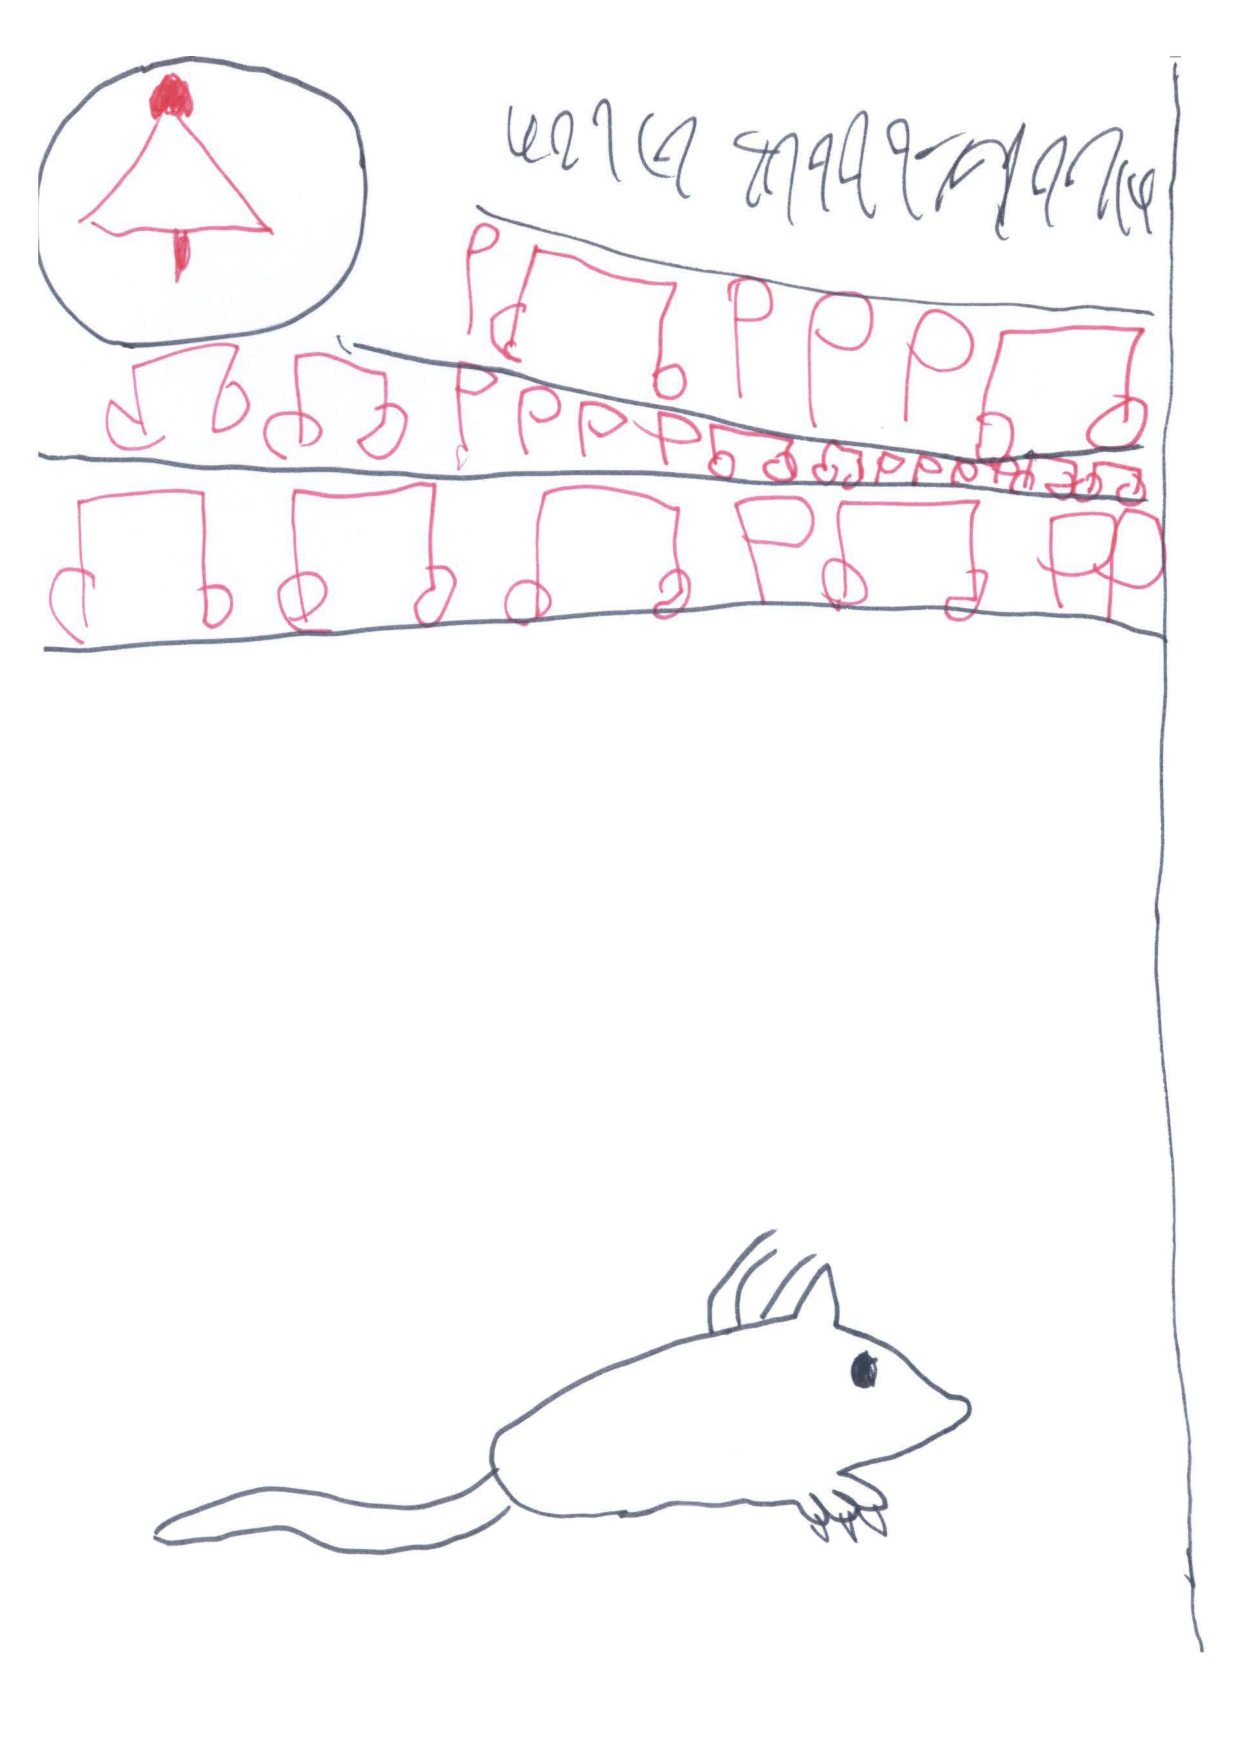
\includegraphics[width=\textwidth]{bilder/maus_2.pdf}
    \end{figure}
    \clearpage
}
Die Maus wanderte weiter und kam an einen Bach, da lebte eine schöne Mäusin. Vornübergebeugt versuchte sie ihre Wäsche im Fluss zu waschen, aber es gelang nicht recht, da sie ihre Pfote nicht richtig bewegen konnte und sie ausserdem furchtbar husten musste. Während die Maus der kranken Mäusin half, erklärte die, schon seit Jahren krank zu sein, aber kein Arzt wisse, wie man ihr helfen könne.

Die Maus fragte auch hier nach Unterkunft und bekam sie. Sie half der armen Mäusin und blieb sogar ein paar Tage, was sie sonst niemals tat. Sie merkte schnell, dass sie gar keine richtige Lust mehr hatte weiter zu reisen. Erst dachte sie, dass es daran liegt, dass sie ja jetzt wisse, welche Frage sie stellen will und ausserdem war vom dicken Bauch nichts mehr übrig. Sie strotzte nur so vor Kraft und Vitalität. Aber sie merkte schnell, dass etwas ganz anderes der Grund ist. Sie hatte sich in die kranke Mäusin verliebt und die wohl auch in sie.

Und am dritten Morgen ging die Maus zum Bach, nahm die Feder und blies sie in die Luft. Als die Feder so hoch war, dass sie über den Wolken schwebte, fragte die Maus, wie wohl der Mäusin zu helfen sei.

Die donnernde Stimme war wieder zu hören und diktierte ein langes Rezept für eine Arzenei. Und sie verordnete Bewegung und frische Luft. Nachdem die Maus den Trunk genau so gebraut hatte und die Mäusin ihn getrunken hatte, fragte die Maus, ob sie Lust hatte, mit ihr durch die Welt zu wandern. Und natürlich wollte die. So nahmen sich die beiden an die Hand und wenn sie nicht angehalten haben, dann wandern sie noch heute. \hfill {\color{DeepPink}\decofourleft}
